\documentclass[a4paper,11pt]{jsarticle}


% 数式
\usepackage{amsmath,amsfonts}
\usepackage{bm}
% 画像
\usepackage[dvipdfmx]{graphicx}
% \usepackage{here}
\usepackage{float}


\begin{document}

\section{演習}
\subsection{(1) サンプリングの限界}
画像の通りの周期でサンプリングを行った。
% \newpage
\begin{figure}[H]
  \centering
  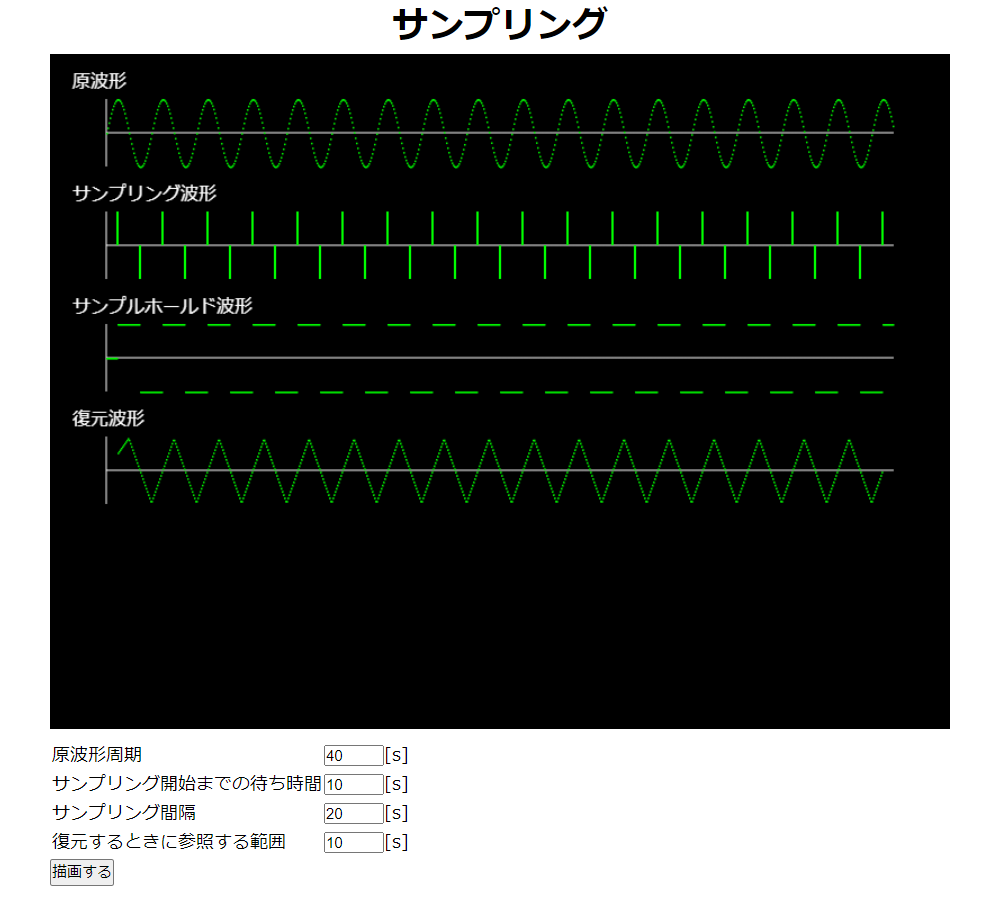
\includegraphics[height=15cm]{./images/sampring_20.png}
  \caption{サンプリング周期 20s}
  \label{fig:sample}
\end{figure}

\begin{figure}[H]
  \centering
  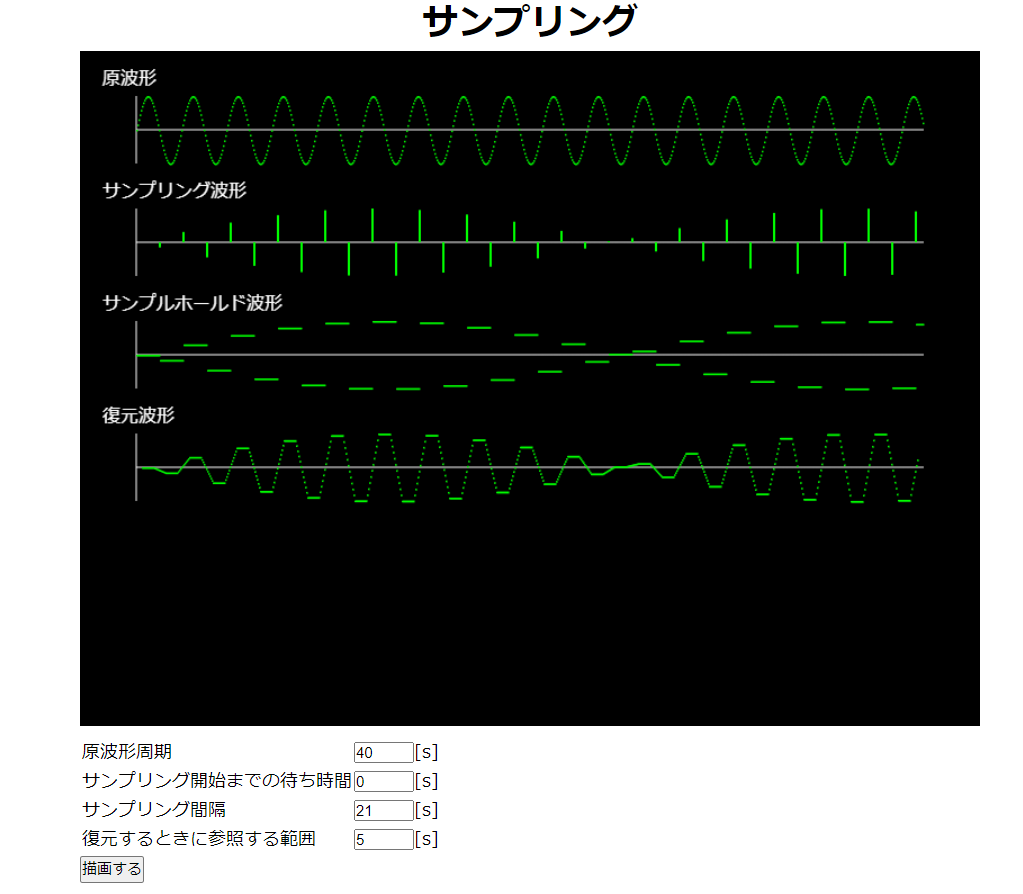
\includegraphics[height=15cm]{./images/sampring_21.png}
  \caption{サンプリング周期 21s}
  \label{fig:sample2}
\end{figure}
\newpage
\subsection{(2) エイリアス}
サンプリング周期を長くするとエイリアスが発生する。

\begin{figure}[H]
  \centering
  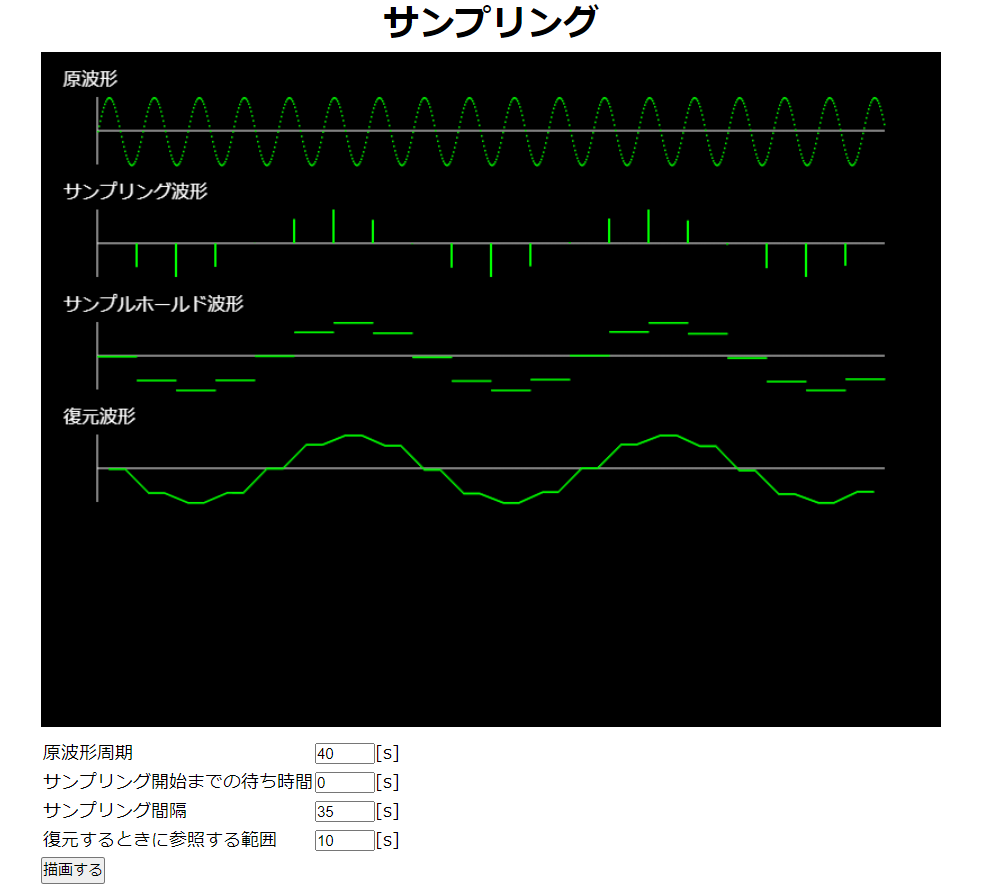
\includegraphics[height=15cm]{./images/エイリアス.png}
  \caption{サンプリング周期 35s}
  \label{fig:sample3}
\end{figure}



\end{document}